The previous section, Section~\ref{sec:data-collection}, described how we collected the clients and libraries, as well as the necessary information to perform our analysis.
In this section, we describe our methodology for detecting and verifying newly added unchecked exceptions in a library when it is updated from an older version to a newer one. Our focus is on identifying the impact of such changes on client code. Specifically, we analyze client programs to detect usage of library methods that were updated to throw previously non-existent unchecked exceptions. Java distinguishes between checked exceptions, which appear as part of method signatures, and unchecked exceptions, which do not. Unchecked exceptions may therefore introduce a class of breaking changes that method signature-based syntactic approaches for Java cannot detect.

After carrying out the data collection steps in Section~\ref{sec:data-collection} and extracting all external library methods invoked by the client, we next analyze their implementations, in both the current version and the latest version. This allows us to compare their behaviour across versions. If we find, through our analysis, that a method now throws a newly added unchecked exception in the latest version, and that the exception can be triggered from the client code, we flag a potential behavioural breaking change. To verify whether this change is in fact breaking, we currently manually write test cases to verify that the client may be affected by the newly introduced exception. We found that this was easy to do given the information that UnCheckGuard reports.

\subsection{Analysis Setup}

\begin{figure*}[hbt!]
    \centering
    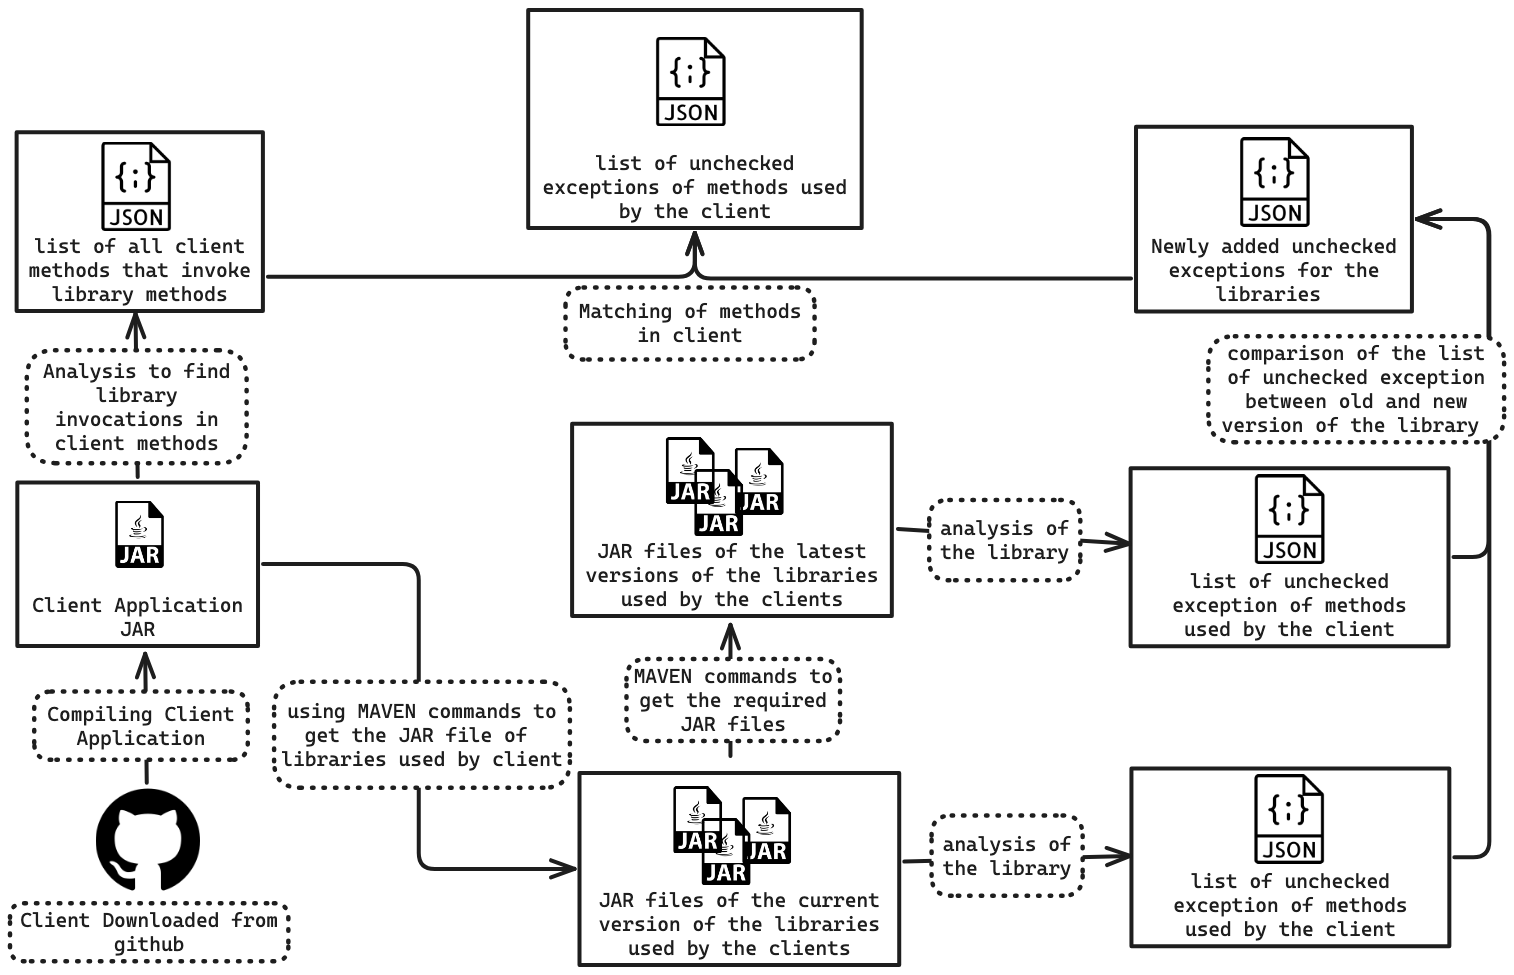
\includegraphics[height=260pt]{diagram/finalPipeline.png}
    \caption{Pipeline of UnCheckGuard for detecting behavioural breaking changes due to newly added unchecked exceptions.}
    \label{fig:jsonjava}
\end{figure*}

The analysis setup is divided into two main phases: client selection and knowledge extraction for analysis. An overview of the full pipeline is shown in Figure~\ref{fig:jsonjava}.

As described in Section~\ref{sec:data-collection}, we begin by selecting Java-based clients from the DUETS dataset~\cite{durieux21:_duets}. We retain only those clients that are Maven-compatible and successfully compile to a JAR file, ensuring compatibility with our analysis tooling.

After selecting the valid clients and compiling them into JAR files, we proceed to extract relevant method-level knowledge from both the client and the current version of the libraries it depends on.

We use SootUp~\cite{Karakaya24:_sootup} to analyze the client JAR and identify all external method invocations. UnCheckGuard performs this analysis by traversing the Jimple intermediate representation of each client method and checking whether any statement contains an \texttt{InvokeExpr}, which represents a method invocation. For each invocation, we retrieve the declaring class type\todo{per our discussion about inheritance, it is possible, though unlikely, that the client invokes on a standard library method and the actual target is in the library.} of the target method. We then check whether this class type is part of the client’s SootUp view---essentially, whether it was declared in the client JAR file or the Java standard library. If the class type is not found in the view, we mark the method as external. This process allows us to filter out internal method calls and focus only on invocations to external library methods.

In parallel, we analyze the current (i.e., pre-upgrade) version of each library used by the client. Using SootUp, we extract all method signatures defined in the library JAR. We then match each external method call made by the client to the corresponding method in the library by comparing their fully qualified method signatures\todo{this doesn't completely work, it's not C, there is dynamic dispatch; for instance, client may have a call to List.add() and library defines LinkedList.add and ArrayList.add() - pending}. This one-to-one mapping enables us to identify exactly which library methods are invoked by which client methods.

At the end of this stage, we produce a structured mapping between client methods and the external library methods they invoke. This mapping serves as a foundation for later stages in our analysis, where we detect behavioural changes in latest library versions and trace their potential impact on client call sites.

\subsection{Finding Newly Added Unchecked Exceptions}

Our primary goal is to detect whether upgrading a library introduces new unchecked exceptions that could affect client behaviour. To achieve this, we divide the process into two stages: first, identifying newly added unchecked exceptions using a call graph; and second, verifying their reachability from client input using a taint analysis.

\subsubsection{Exception Discovery with RTA}

To detect newly added unchecked exceptions in the latest library versions, we first construct a call graph using Rapid Type Analysis~\cite{bacon96:_fast_static_analy_c_virtual_funct_calls} (RTA) via SootUp~\cite{Karakaya24:_sootup}. We use RTA instead of Class Hierarchy Analysis (CHA) because RTA provides a more precise approximation of runtime behaviour in the context of a particular client/library pair. CHA, working on the class hierarchy, includes all methods defined in subclasses and interface implementations regardless of whether they are actually invoked. RTA instead considers only those types that are instantiated in the program (client plus libraries), resulting in a more accurate call graph.

By definition, CHA reports the most conservative soundy~\cite{livshits15:_in} answer possible, absent reflection and other dynamic features. Thus, it tends to over-approximate and report unreachable method calls. For example, in one case, CHA identified a path from the public \texttt{getString(String)}\footnote{Fully-qualified name: method \texttt{getString(String)} returning a \texttt{String} on class \texttt{com.alibaba.fastjson.JSONObject}} method, reporting an exception thrown in the \texttt{JSONObject} constructor as reachable. However, manual inspection revealed that this path was spurious—the method \texttt{getString} never reaches the constructor in question because, in the specific program under analysis, no code instantiates a \texttt{JSONObject}. RTA excludes such paths because it considers only types that are actually instantiated, whereas CHA includes all potential subtype relationships, regardless of runtime feasibility.
% we should probably make this whole discussion more concise when we have space limitations

After building the RTA-based call graph, we traverse the entire callgraph and collect all exceptions that are subclasses of \texttt{java.lang.RuntimeException} or \texttt{java.lang.Error}. Per the definition of the Java programming language, such exceptions represent the complete set of unchecked exceptions that the client might be newly exposed to due to the library upgrade.

\subsubsection{Exception Filtering with Taint Analysis}

Once we collect the list of unchecked exceptions, we need to determine which of them can actually be triggered by client inputs. This is necessary because many exceptions that show up during call graph analysis are not reachable in practice—they rely on internal values rather than any parameters the client supplies. To filter out such cases, we use FlowDroid~\cite{Arzt14:_flowdroid}, a static taint analysis framework.

Consider the following case drawn from our corpus. The client \texttt{4ntoine/ServiceDiscovery-java}\footnote{\url{https://github.com/4ntoine/ServiceDiscovery-java}} uses the method \texttt{copyFromUtf8(String)} from the library \texttt{protobuf-java-2.6.1}. When this library is upgraded to \texttt{protobuf-java-4.30.1}, the method's implementation adds a new unchecked exception—an \texttt{IllegalArgumentException}. Our tool initially flags this as a behavioural breaking change because the exception is present in the latest version and not in the current one, and because there is a interprocedural control-flow path from the client method to the callsite where the exception is thrown.

However, a closer inspection shows that this exception cannot be triggered by any value passed from the client. The method that throws the exception looks like this:

\begin{lstlisting}[language=Java,breaklines=true,basicstyle=\scriptsize\ttfamily]
static CodedInputStream newInstance(
    final byte[] buf, final int off, final int len, final boolean bufferIsImmutable) {
  ArrayDecoder result = new ArrayDecoder(buf, off, len, bufferIsImmutable);
  try {
    result.pushLimit(len);
  } catch (InvalidProtocolBufferException ex) {
    // The only reason pushLimit() might throw an exception
    // here is if len is negative. Normally pushLimit()'s
    // parameter comes directly off the wire, so it's 
    // important to catch exceptions in case of corrupt or
    // malicious data. However, in this case, we expect 
    // that len is not a user-supplied value, so we can 
    // assume that it being negative indicates a 
    // programming error. Therefore, throwing an unchecked 
    // exception is appropriate.
    throw new IllegalArgumentException(ex);
  }
  return result;
}
\end{lstlisting}

In the comment written by the library developer, the developer states that this exception cannot be thrown by this non-public method, essentially because \texttt{len} cannot be directly supplied by a client. Clients can only reach this \texttt{newInstance} method by initially calling methods that are part of \texttt{protobuf}'s API. Our taint analysis confirms that no user-supplied value (source) flows from the client into the \texttt{IllegalArgumentException} constructor (sink). We choose exception constructors as sinks because taintedness of the exception constructor means that the client-controlled value can affect the reachability of the exception, i.e. whether the exception might be thrown or not. Hence, taint analysis helps reason about whether the exception can actually cause a behavioural breaking change in the client.

For technical FlowDroid-related reasons, we automatically generate a \textit{driver stub} for each value that the client supplies to the library. To our knowledge, FlowDroid does not allow marking method parameters directly as sources. Instead, we wrap each parameter in a synthetic method whose return value is marked as a source. This approach allows us to simulate tainted inputs and track their flow through the library method. Stub generation, implemented using SootUp, handles a variety of cases, including:
\begin{itemize}
  \item Constructor methods (\texttt{<init>} using \texttt{new ClassName(...)})
  \item Static and instance methods
  \item Void and non-void return types
  \item Primitive parameters (e.g., \texttt{int} $\rightarrow$ \texttt{0})
  \item Object parameters (defaulted to \texttt{null})
  \item Nested classes (converting \texttt{\$} to \texttt{.})
  \item Multiple parameters (sources named \texttt{SourceN()}, where $N$ is the parameter index)
  \item Overloaded methods (only one version retained)
\end{itemize}

An example of a driver stub follows.
\begin{lstlisting}[language=Java,breaklines=true,breakatwhitespace=false,basicstyle=\scriptsize\ttfamily]
public class DriverStub {
    public static java.lang.String source0() {
        return null;
    }

    public static void run() {
        int result = new com.alibaba.fastjson.JSONObject().getIntValue(source0());
    }
}
\end{lstlisting}

In the above example of the driver stub, we generate a stub for library \texttt{fastjson-1.2.58}'s public \texttt{getIntValue(String)} method\footnote{Fully-qualified name: method \texttt{getIntValue(String)}, returning a \texttt{int} on class \texttt{com.alibaba.fastjson.JSONObject}}. This method has a \texttt{java.lang.String} parameter. We therefore declare a method named \texttt{source0} in the driver stub, and declare that method to be a source; FlowDroid then marks its return value as a source. We generate the way \texttt{getIntValue} is called based on the type of method it is, and obtain the properties of the method using SootUp.

We treat each exception discovered in the RTA phase as a \textit{taint sink}. For this analysis, we intentionally construct the call graph using Class Hierarchy Analysis (CHA). Although CHA is less precise than RTA, it offers conservative coverage, reducing the risk of missing true positive flows due to aggressive pruning.

Consider the following method from the \texttt{beam-sdks-java-core} library:

\begin{lstlisting}[language=Java,breaklines=true,breakatwhitespace=false,basicstyle=\scriptsize\ttfamily]
public static void applicableTo(PCollection<?> input) {
 WindowingStrategy<?, ?> ws = input.getWindowingStrategy();
 if (ws.getWindowFn() instanceof GlobalWindows
     && ws.getTrigger() instanceof DefaultTrigger
     && input.isBounded() != IsBounded.BOUNDED) {
  throw new IllegalStateException("...");
 }
}
\end{lstlisting}

\begin{figure}[t]
\centering
\scalebox{0.75}{
\begin{tikzpicture}[
  node distance=1.4cm and 1.5cm,
  box/.style={rectangle, draw, rounded corners, minimum height=1.2em, text width=2.8cm, align=center, font=\scriptsize},
  every edge/.style={draw, -{Latex[width=2mm]}},
  rededge/.style={draw=red, thick, dashed, -{Latex[width=2mm]}}
  ]

% Nodes
\node[box] (start) {\textbf{Method Entry}\\ \texttt{applicableTo(...)}};
\node[box, below=of start] (cond) {\textbf{Condition}\\ \texttt{input.isBounded() != BOUNDED}};
\node[box, below left=of cond] (exc) {Throws \\ \texttt{IllegalStateExcep...}};
\node[box, below right=of cond] (noexc) {Execution continues};

% Edges
\path (start) edge (cond);
\path (cond) edge (exc);
\path (cond) edge (noexc);

% Labels
\node[align=left, font=\scriptsize] at ([xshift=1.9cm,yshift=0.1cm]cond.east) {\textbf{CHA:} includes both branches};
\draw[rededge] (start.east) to[out=10,in=90] node[right, align=center, font=\scriptsize] {\textbf{RTA:} skips method due to\\ uninstantiated classes} (noexc.west);

\end{tikzpicture}
}
\vspace{-1ex}
\caption{CHA vs. RTA: RTA only reaches the \texttt{IllegalStateException} if types like \texttt{GlobalWindows} or \texttt{DefaultTrigger} are instantiated in the analyzed code.}
\label{fig:rta-vs-cha}
\vspace{-2ex}
\end{figure}


In this example, the parameter \texttt{input} is the taint source, and the \texttt{IllegalStateException} is the sink. The public \texttt{applicableTo(PCollection)}\footnote{Fully-qualified name: method \texttt{applicableTo(PCollection)} returning a \texttt{void} on class \texttt{org.apache.beam.sdk.transforms.GroupByKe}} method is used by the \texttt{0xdecaf/beam-enrichment-patterns}\footnote{\url{github.com/0xdecaf/beam-enrichment-patterns}} client.

RTA excludes types that are never instantiated in the analyzed program. It is more precise and reaches the exception only if actual runtime types lead to the throw statement. In contrast, CHA is more conservative. In this case, RTA reaches the \texttt{IllegalStateException} only if classes such as \texttt{GlobalWindows} or \texttt{DefaultTrigger} are instantiated in the analyzed codebase. CHA, on the other hand, includes all possible overrides regardless of whether those types are instantiated. As a result, even if the actual runtime types are unused, CHA still explores all feasible paths and reaches the IllegalStateException. As shown in Figure~\ref{fig:rta-vs-cha}, this broader approximation allows taint analysis to identify exception flows that RTA would miss due to its stricter instantiation-based filtering.\todo{I still don't believe this: if GlobalWindows or DefaultTrigger are never invoked, why does it matter?}

% RTA excludes types that are never instantiated in the analyzed program. As a result, if no code in the client or the library instantiates a \texttt{PCollection}, the method \texttt{applicableTo(PCollection)} may not appear in the RTA-generated call graph at all. This exclusion causes the exception thrown in that method to be missed. In contrast, CHA includes all types from the class hierarchy regardless of instantiation, so the method is included in the call graph along with the conditional path to the exception. As shown in Figure~\ref{fig:rta-vs-cha}, this broader approximation allows the taint analysis to identify exception flows that RTA would miss due to its stricter instantiation-based filtering.

This trade-off justifies the use of CHA in the filtering phase: although it may over-approximate in some cases, it ensures that no critical exception flows are missed.

After collecting the list of unchecked exceptions for each method in both the old and latest versions of the library, we perform a comparison to identify newly introduced exceptions. If a method exists in the old version but is missing from the latest version, we exclude it from our analysis, as its removal may indicate a method signature–based breaking change, which is handled by existing tools and lies outside the scope of our detection.

For methods that appear in both versions, we compare the sets of unchecked exceptions that they throw. We perform this comparison using both the exception type (e.g., \texttt{java.lang.IllegalArgumentException}) and the fully qualified signature of the method in which the exception occurs. If, after removing all exceptions common to both versions, the method in the latest version still contains any additional unchecked exceptions, we classify it as a method with a newly added unchecked exception. Otherwise, we discard it from further consideration; our technique cannot find new exception-related behavioural breaking changes for this library method.

\subsection{Filtering Untriggerable Unchecked Exceptions}

Based on the information collected about newly added unchecked exceptions, we use the previously generated client-to-library method mapping to determine which client methods invoke a library method that now throws a new unchecked exception. This step allows us to identify specific client call sites that may be affected by behavioural breaking changes introduced in the upgraded library version.

To validate the practical impact of these changes, we manually write test cases to assess whether the client can actually trigger the exception. Each test case is constructed starting from the client call site identified in the mapping. We then examine the method that was flagged as containing a newly added unchecked exception. This information is available in the JSON output produced by our tool, which includes the exception type and the method signature in which it occurs.

The JSON output helps us locate the exact exception-throwing line in the library, which enables a detailed inspection of how the exception is triggered. We first test the exception by directly calling the relevant library method with crafted parameters. If this call triggers the exception, we proceed to construct a full test case that invokes the client method, propagating the same parameter values.

In some scenarios, we are unable to trigger the exception through the client due to certain code structures:
\begin{itemize}
  \item The client may pass down a hardcoded constant value, which does not trigger the exception.
  \item The client may apply explicit guards or checks before calling the affected library method.
\end{itemize}

This is similar in spirit to, for instance, security tools which report a number of potential vulnerabilities; the onus remains on the tool user to go from a potential vulnerability to proof-of-concept code.

Even in cases where no test case could possibly trigger the exception, the information produced by our tool remains useful for the client developer, as future code changes (e.g., modifying a hardcoded value or removing a check) could make the call site vulnerable to the newly introduced exception. The library developer ought to add a description of this exception, and the circumstances under which it could be thrown, to the library method's documentation.

For example, in the client project \texttt{github.com/4ntoine/ServiceDiscovery-java}, we analyze the following code:

\begin{lstlisting}[language=Java, basicstyle=\scriptsize\ttfamily, breaklines=true]
if (serviceInfo.getPayload() != null)
    builder.setPayload(ByteString.copyFrom(serviceInfo.getPayload()));
\end{lstlisting}

In this case, the method with the newly added unchecked exception is:

\begin{lstlisting}[language=Java, basicstyle=\scriptsize\ttfamily]
com.google.protobuf.ByteString.copyFrom(byte[])
\end{lstlisting}

The client uses version 2.6.1 of \texttt{protobuf-java}, while the latest version is 4.31.0. The newly added exception, \texttt{java.lang.NullPointerException}, is thrown in the latest library if a null value is passed to \texttt{copyFrom}. The relevant code from the library looks like this:

\begin{lstlisting}[language=Java, basicstyle=\scriptsize\ttfamily]
LiteralByteString(byte[] bytes) {
    if (bytes == null) {
        throw new NullPointerException();
    }
    this.bytes = bytes;
}
\end{lstlisting}

Although the latest version introduces a new unchecked exception, the client has already placed a guard condition:

\begin{lstlisting}[language=Java, basicstyle=\scriptsize\ttfamily]
if (serviceInfo.getPayload() != null)
\end{lstlisting}

This prevents the exception from being triggered. Therefore, we cannot generate a test case for this call site, but we still report it as potentially relevant.

In contrast, for cases where the client does not enforce such conditions and passes input parameters that can trigger the new exception, we can generate a test case to demonstrate the behavioural breaking change. In these situations, the change is not merely hypothetical—it represents an actual, runtime-breaking behaviour that occurs when the latest library is used. These tests offer actionable insights to developers by highlighting call sites could possibly trigger newly added exceptions in new library versions.


